\section{Grupo Fundamental}
\label{grupo-fundamental}

\begin{titlemize}{Lista de Dependências}
	\item \hyperref[homotopia]{Homotopia}\\ %homotopia
\end{titlemize}

Considere um espaço topológico com um ponto base fixado. O seu grupo fundamental é o grupo das classes de equivalência (sob homotopia relativa aos extremos) dos laços no espaço saindo do ponto base. Tal grupo armazena certas informações sobre buracos do espaço topologico, e é invariante sobre a equivalência homotópica. Esta é uma ferramenta poderosa para verificar se dois espaços topológicos são homeomorfos. % (homotópicos). %retirei, não entendi o que querem dizer
Veremos como sua construção se dá com mais detalhes.

%---------------------------------------------------------------------------------------------------------------------!Draft!-----------------------------------------------------------------------------------------------------------------
\subsection{Espaço de Laços}
\label{espaco-lacos-def}
\begin{titlemize}{Lista de dependências}
	%\item \hyperref[dependecia1]{Dependência 1};\\ %'dependencia1' é o label onde o conceito Dependência 1 aparece (--à arrumar um padrão para referencias e labels--)
    \item \hyperref[homotopia-relativa-def]{Homotopia Relativa}
	\item \hyperref[homotopia-relaçao-de-equivalencia-prop]{Homotopia é relação de equivalência};\\
% quantas dependências forem necessárias.
\end{titlemize}
\begin{defi}[Espaço de Laços]
	Seja $X$ um espaço topológico e seja $x_0\in X$ um ponto base. O \textbf{espaço de laços} em $X$ que saem de $x_0$ é definido como
\[\Omega(X,x_0) = \left\{\gamma: I \to X ~|~ \gamma\text{ é contínua e }\gamma(0)=\gamma(1)=x_0\right\}.\]
\end{defi}

Investigaremos a fundo o conjunto $\pi_1(X,x_0) = \Omega(X,x_0)/\sim$, onde $\alpha \sim \beta$ se, e somente se, $\alpha$ e $\beta$ são homotópicas relativo a $\partial I = \{0,1\}$.

\begin{titlemize}{Lista de consequências}
	\item \hyperref[homotopia-relaçao-de-equivalencia]{Homotopia como relação de equivalência};\\ %'consequencia1' é o label onde o conceito Consequência 1 aparece
	\item \hyperref[homotopia-teorema-da-bola-cabeluda]{Teorema da bola cabeluda}
\end{titlemize}

%[Bianca]: é mais fácil criar a lista de dependências do que a de consequências.
\subsection{Produto concatenação de caminhos}
\label{Produto-concatenacao-def}
%\begin{titlemize}{Lista de dependências}
	%\item \hyperref[dependecia1]{Dependência 1};\\ % homotopia
%\end{titlemize}
\begin{defi}[Concatenação de caminhos]
	Seja $X$ um espaço topológico, e sejam $\alpha:I\rightarrow X, \beta:I\rightarrow X$ duas funções contínuas tal que $\beta(0)=\alpha(1).$ O produto concatenação de $\alpha$ e $\beta$ é uma função contínua $\alpha*\beta:I\rightarrow X$ dada por 
 \begin{align*}
     (\alpha*\beta)(s)=\begin{cases}
         \alpha(2s)\mbox{ se }0\le s\le\frac{1}{2}\\
         \beta(2s-1)\mbox{ se }\frac{1}{2}\le s \le 1
     \end{cases}
 \end{align*}
\end{defi}

Esse produto será usado para definir o grupo fundamental.

\begin{titlemize}{Lista de consequências}
	%\item \hyperref[consequencia1]{Consequência 1};\\ %'consequencia1' é o label onde o conceito Consequência 1 aparece
	\item \hyperref[produto-bem-definido-prop]{O produto do grupo fundamental}
\end{titlemize}

%[Bianca]: é mais fácil criar a lista de dependências do que a de consequências.

\subsection{O produto do grupo fundamental} %afirmação aqui significa teorema/proposição/colorário/lema
\label{produto-bem-definido-prop}
\begin{titlemize}{Lista de dependências}
	\item \hyperref[Produto-concatenacao-def]{Produto concatenação de caminhos};\\ %'dependencia1' é o label onde o conceito Dependência 1 aparece (--à arrumar um padrão para referencias e labels--) 
% quantas dependências forem necessárias.
\end{titlemize}
Sejam $X$ um espaço topológico e $x_0\in X$. Provemos que o produto concatenação induz um produto $\cdot$ (operação binária) no espaço quociente $\pi_1(X,x_0)$, e que, além disso, $(\pi_1(X,x_0),\cdot)$ é um grupo.

\begin{lemma}% ou af(afirmação)/prop(proposição)/corol(corolário)/lemma(lema)/outros ambientes devem ser definidos no preambulo de Alg.Top-Wiki.tex 
    O produto $\cdot:\pi_1(X,x_0)\times\pi_1(X,x_0)\rightarrow \pi_1(X,x_0)$ dado por $[\alpha]\cdot[\beta]=[\alpha*\beta]$ é bem definido.
\end{lemma}

\begin{dem}
    É claro que o produto concatenação de dois laços em $\Omega(X,x_0)$ ainda é um laço em $\Omega(X,x_0)$. Basta provar que o produto $\cdot$ não depende da escolha de representantes. Sejam $\alpha\sim_H \alpha'$ e $\beta\sim_G\beta'$ laços em $\Omega(X,x_0)$. Então, a função $H*G:I\times I\rightarrow X$ dada por 
    \begin{align*}
        H*G(s,t)=\begin{cases}
            H(2s,t)\qquad&\mbox{ se }0\le s\le \frac{1}{2}\\
            G(2s-1,t)\qquad&\mbox{ se }\frac{1}{2}\le s\le1
        \end{cases}
    \end{align*}
    é uma homotopia satisfazendo $H*G(s,0)=\alpha*\beta(s),$ $H*G(s,1)=\alpha'*\beta'(s)$ e $H*G(0,t)=H*G(1,t)=x_0$ para todos $s,t\in I$. Ou seja, $H*G$ é uma homotopia relativa à $\partial I$ entre $(\alpha*\beta)$ e $(\alpha'*\beta').$ Logo, temos  
    $$[\alpha]\cdot[\beta]=[\alpha*\beta]=[\alpha'*\beta']=[\alpha']\cdot [\beta']$$
    conforme desejado.
\end{dem}

\begin{lemma}
    O produto $\cdot$ é associativo. Ou seja, para todos $\alpha,\beta,\gamma\in\Omega(X,x_0),$ vale
    \[(\alpha*\beta)*\gamma\sim \alpha*(\beta*\gamma).\]
\end{lemma}

\begin{dem}
    Basta exibir uma homotopia entre tais laços. Definimos a função $H:I\times I\rightarrow X$ na seguinte forma:
    \begin{align*}
        H(s,t)=\begin{cases}
            \alpha(\frac{4s}{t+1})\qquad &\mbox{ se }0\le s \le \frac{t+1}{4}\\
            \beta(4s-t-1)\qquad &\mbox{ se }\frac{t+1}{4}\le s\le\frac{t+2}{4}\\
            \gamma(\frac{4s-t-2}{2-t})\qquad &\mbox{ se }\frac{t+2}{4}\le s\le 1.
        \end{cases}
    \end{align*}
    É fácil ver que $H$ é uma homotopia que satisfaz
    \begin{align*}
        H(s,0)=\begin{cases}
            \alpha(\frac{4s}{1})\qquad &\mbox{ se }0\le s \le \frac{1}{4}\\
            \beta(4s-1)\qquad &\mbox{ se }\frac{1}{4}\le s\le\frac{2}{4}\\
            \gamma(\frac{4s-2}{2})\qquad &\mbox{ se }\frac{2}{4}\le s\le 1.
        \end{cases}\quad=((\alpha*\beta)*\gamma)(s),
    \end{align*}
    \begin{align*}
        H(s,1)=\begin{cases}
            \alpha(\frac{4s}{2})\qquad &\mbox{ se }0\le s \le \frac{2}{4}\\
            \beta(4s-2)\qquad &\mbox{ se }\frac{2}{4}\le s\le\frac{3}{4}\\
            \gamma(4s-3)\qquad &\mbox{ se }\frac{3}{4}\le s\le 1.
        \end{cases}\quad=(\alpha*(\beta*\gamma))(s)
    \end{align*}
    e $H(0,t)=H(1,t)=x_0.$ Portanto, $$(\alpha*\beta)*\gamma\sim \alpha*(\beta*\gamma)$$ conforme desejado.
\end{dem}

\begin{lemma}
    Seja $c_{x_0}:I\rightarrow X$ uma função constante cuja valor é igual a $x_0.$ Então, para todo laço $\alpha\in \Omega(X,x_0),$ vale
    $$c_{x_0}*\alpha\sim\alpha\sim\alpha*c_{x_0}.$$
    Ou seja, $[c_{x_0}]$ é o elemento neutro em $(\pi_1(X,x_0),\cdot)$.
\end{lemma}

\begin{dem}
    A homotopia $H$ dada por 
    \begin{align*}
        H(s,t)=\begin{cases}
            x_0\qquad &\mbox{ se }0\le s \le \frac{1-t}{2}\\
            \alpha(\frac{2s-1+t}{1+t}) \qquad &\mbox{ se }\frac{1-t}{2}\le s\le 1
        \end{cases}
    \end{align*}
    é uma homotopia relativa à $\partial I$ entre $c_{x_0}*\alpha$ e $\alpha.$
    
    A homotopia $G$ dada por 
    \begin{align*}
        G(s,t)=\begin{cases}
            \alpha(\frac{2s}{t+1})\qquad &\mbox{ se }0\le s \le \frac{t+1}{2}\\
            x_0\qquad &\mbox{ se }\frac{t+1}{2}\le s \le 1
        \end{cases}
    \end{align*}
    é uma homotopia relativa à $\partial I$ entre $\alpha*c_{x_0}$ e $\alpha.$ Portanto, $$c_{x_0}*\alpha\sim\alpha\sim\alpha*c_{x_0},$$ como queríamos demonstrar.
\end{dem}

\begin{lemma}
    Dado um laço $\alpha \in \Omega(X,x_0)$, vale que $\overline{\alpha}$ dado por $\overline{\alpha}(s)=\alpha(1-s)$ é um laço satisfazendo 
    $$\overline{\alpha}*\alpha\sim c_{x_0}=\alpha*\overline{\alpha}.$$
    Ou seja, $[\overline{\alpha}]$ é o elemento inverso de $[\alpha]$ em $(\pi_1(X,x_0),\cdot)$.
\end{lemma}

\begin{dem}
    A homotopia $H$ dada por 
    \begin{align*}
        H(s,t)=\begin{cases}
            \overline{\alpha}(2s(1-t))\qquad &\mbox{ se }0\le s \le \frac{1}{2}\\
            \overline{\alpha}(2(1-s)(1-t)) \qquad &\mbox{ se }\frac{1}{2}\le s\le 1 
        \end{cases}
    \end{align*}
    é uma homotopia relativa à $\partial I$ entre $\overline{\alpha}*\alpha$ e $c_{x_0},$ porque $H(s,1)=\overline{\alpha}(0)=x_0$ para todo $s\in I$ e 
    \begin{align*}
        H(s,0)=\begin{cases}
            \overline{\alpha}(2s)\qquad &\mbox{ se }0\le s \le \frac{1}{2}\\
            \overline{\alpha}(2(1-s))=\alpha(2s-1) \qquad &\mbox{ se }\frac{1}{2}\le s\le 1
        \end{cases}
    \end{align*}
    (Geometricamente, $H(s,t_0)$ é um laço que anda em $\alpha(s),$ para num certo ponto e faz o caminho de volta).
    De forma análoga, a homotopia $G$ dada por 
   
\begin{align*}
        H(s,t)=\begin{cases}
            \alpha(2s(1-t))\qquad &\mbox{ se }0\le s \le \frac{1}{2} \\
            \alpha(2(1-s)(1-t)) \qquad &\mbox{ se }\frac{1}{2}\le s\le 1 
        \end{cases}
    \end{align*}
    é uma homotopia relativa à $\partial I$ entre $\alpha*\overline{\alpha}$ e $c_{x_0}.$ Portanto, $$\overline{\alpha}*\alpha\sim c_{x_0}=\alpha*\overline{\alpha}$$ conforme desejado.
\end{dem}

Juntando todos os lemas, concluímos: 

\begin{thm}
    Dados $X$ um espaço topológico e $x_0\in X$, vale que $(\pi_1(X,x_0),\cdot)$ é um grupo.
\end{thm}

\begin{titlemize}{Lista de consequências}
	\item \hyperref[grupo-fundamental-def]{Grupo fundamental};\\
    \item \hyperref[conjugacao-por-curva-prop]{Conjugação por uma Curva}
\end{titlemize}

\subsection{Grupo fundamental}
\label{grupo-fundamental-def}
\begin{titlemize}{Lista de dependências}
	\item \hyperref[espaco-lacos-def]{O espaço de laços}
	\item \hyperref[produto-bem-definido-prop]{O produto do grupo fundamental};\\ %'dependencia1' é o label onde o conceito Dependência 1 aparece (--à arrumar um padrão para referencias e labels--) 
% quantas dependências forem necessárias.
\end{titlemize}
\begin{defi}[Grupo fundamental]
	Seja $X$ um espaço topológico e seja $x_0$ um ponto de $X.$ O grupo fundamental de $X$ em $x_0$ é $(\pi_1(X,x_0),\cdot)$, onde $\pi_1(X,x_0) = \Omega(X,x_0)/\sim$, onde $\alpha \sim \beta$ se, e somente se, $\alpha$ e $\beta$ são homotópicas relativo aos extremos, e o produto $\cdot$ é dado por $[\alpha]\cdot\[\beta\] = [\alpha \cdot \beta]$, em que $\alpha \cdot \beta$ é a concatenação de $\alpha$ e $\beta$.
\end{defi}

No geral, o grupo fundamental depende da escolha do ponto base $x_0$.

\begin{titlemize}{Lista de consequências}
	\item \hyperref[hom-grupo-fundamental]{Homomorfismo induzido};\\ %'consequencia1' é o label onde o conceito Consequência 1 aparece
	\item \hyperref[]{}
\end{titlemize}

\subsection{Homomorfismo de grupo fundamental}
\label{hom-grupo-fundamental}
\begin{titlemize}{Lista de dependências}
	\item \hyperref[grupo-fundamental-def]{Dependência 1};\\ %'dependencia1' é o label onde o conceito Dependência 1 aparece (--à arrumar um padrão para referencias e labels--) 
\end{titlemize}
Sejam $X,Y$ espaços topológicos não triviais e $f:X\rightarrow Y$ uma função contínua. Então, $f$ induz uma função entre grupos fundamentais de forma natural:
\begin{align*}
    f_*:\pi_1(X,x_0)&\longrightarrow\pi_1(Y,f(x_0))\\
    [\alpha]\longmapsto [f\circ \alpha].
\end{align*}
É fácil de observar que $f_*$ está bem definida pois se $\alpha\sim \alpha'$ relativa à $\partial I,$ então $f\circ \alpha\sim f\circ \alpha'$ relativa à $\partial I.$ Além disso, se $f\sim g$ relativa à $\partial I$, então $f_*=g_*.$ Agora, provaremos que $f_*$ é um homomorfismo de grupo.
\begin{prop}
    Sejam $X,Y,Z$ espaços topológicos não triviais, e sejam $f:(X,x_0)\rightarrow (Y,y_0)$ e $g:(Y,y_0)\rightarrow (Z,z_0)$ duas funções contínuas que satisfazem $f(x_0)=y_0$ e $g(y_0)=z_0.$ Então, 
    \begin{itemize}
        \item $g_*\circ f_*=(g\circ f)_*;$
        \item $(1_X)_*=1_{\pi_1(X,x_0)};$
        \item $f_*$ é homomorfismo de grupos.
    \end{itemize}
\end{prop}
    
\begin{dem}
    Os dois primeiros itens são triviais. Vamos provar que $f_*$ é homomorfismo. Primeiramente note que 
    \begin{align*}
        f\circ (\alpha*\beta)(s)=\begin{cases}
            f(\alpha(2s))&\;\;\;\mbox{ se }0\le s\le \frac{1}{2}\\
            f(\beta(2s-1))&\;\;\;\mbox{ se }\frac{1}{2}\le s\le 1
        \end{cases}\;\;\;\;= ((f\circ\alpha)*(f\circ \beta))(s)
    \end{align*}
    Logo, temos
    \begin{align*}
        f_*([\alpha]\cdot [\beta])=f_*[\alpha*\beta]=[f\circ (\alpha*\beta)]=[(f\circ\alpha)*(f\circ\beta)]=(f_*[\alpha])\cdot (f_*[\beta])
    \end{align*}
    conforme desejado.
\end{dem}

Podemos concluir que na linguagem da teoria de categorias, $\pi_1$ é um funtor de $\textbf{Top}^*$ em \textbf{Gr}. 

Como consequência, temos que $\pi_1(X,x_0)$ é invariante topológico.

\begin{corol}
    Se $f:X\rightarrow Y$ é homeomorfismo, então $f_*:\pi_1 (X,x_0)\rightarrow \pi_1(Y,f(x_0))$ é um isomorfismo de grupos.
\end{corol}

\begin{dem}
    Seja $g:Y\rightarrow X$ a inversa de $f.$ Pela proposição anterior, temos que 
    $$f_*\circ g_*=(f\circ g)_*=(1_Y)_*=1_{\pi_1(Y,f(x_0))}$$
    e 
    $$g_*\circ f_*=(g\circ f)_*=(1_X)_*=1_{\pi_1 (X,x_0)}.$$
    Portanto, $f_*$ é um isomorfismo de grupo.
\end{dem}

\begin{titlemize}{Lista de consequências}
	\item \hyperref[consequencia1]{Consequência 1};\\ %'consequencia1' é o label onde o conceito Consequência 1 aparece
	\item \hyperref[]{}
\end{titlemize}

%---------------------------------------------------------------------------------------------------------------------!Draft!-----------------------------------------------------------------------------------------------------------------
\subsection{Conjugação por uma Curva} %[conjugacao-por-curva-prop]{Conjugação por uma Curva}
\label{conjugacao-por-curva-prop}
\begin{titlemize}{Lista de dependências}
    \item \hyperref[espaco-lacos-def]{Espaço de Laços};\\
    \item \hyperref[produto-bem-definido-prop]{O produto do grupo fundamental};\\
	\item \hyperref[grupo-fundamental-def]{O Grupo Fundamental};
% quantas dependências forem necessárias.
\end{titlemize}
%Comentário sobre os objetos envolvidos na afirmação.
\begin{defi}[Conjugação de laços por uma curva] 
	Sejam $x_0$ e $x_1$ pontos em um espaço topológico $X$ e seja $\gamma: I \to X$ uma curva contínua ligando $x_0$ a $x_1$; isto é, $\gamma(0)=x_0$ e $\gamma(1) = x_1$. Seja também $\eta \in \Omega(X,x_0)$ um laço saindo de $x_0$. Definimos a conjugação de $\eta$ por $\gamma$ como $\overline{\gamma} * \eta * \gamma \in \Omega(X,x_1)$, laço saindo de $x_1$. Isto define uma função $A_{\gamma}: \Omega(X,x_0) \to \Omega(X,x_1)$.
\end{defi}

\begin{prop}[Isomorfismo de grupos induzido por $A_{\gamma}$]
    Sejam $x_0$ e $x_1$ pontos em um espaço topológico $X$ e seja $\gamma: I \to X$ uma curva ligando $x_0$ a $x_1$.
    
    Então $A_{\gamma}$ induz um isomorfismo de grupos \begin{align*}
        \hat{A}_{\gamma}: \pi_1(X,x_0)&\to \pi_1(X,x_1)\\
        \hat{A}_{\gamma}([\eta]) &= [A_{\gamma}(\eta)] = [\overline{\gamma} * \eta * \gamma].
    \end{align*}

    \begin{dem}
        Provemos primeiramente que $\hat{A}_{\gamma}$ está bem definida. Considere $c_{\gamma}: \gamma \Rightarrow \gamma$ e $c_{\overline{\gamma}}: \overline{\gamma} \Rightarrow \overline{\gamma}$ as homotopias constantes. Assim, se $\eta, \nu \in \Omega(X,x_0)$ e $H: \eta \Rightarrow \nu$ é uma homotopia relativa a $\partial I$ então é claro que $c_{\overline{\gamma}}*H*c_{\gamma}: A_{\gamma}(\eta) \Rightarrow A_{\gamma}(\nu)$ também é homotopia relativa a $\partial I$.

        $\hat{A}_{\gamma}$ é um homomorfismo de grupos, já que dadas $\eta, \nu \in \Omega(X,x_0)$,
        \begin{align*}
            \hat{A}_{\gamma}([\eta]\cdot[\nu]^{-1})
            &= \hat{A}_{\gamma}([\eta * \overline{\nu}])\\
            &= [\overline{\gamma} * (\eta * \overline{\nu}) * \gamma]\\
            &= [(\overline{\gamma} * \eta * \gamma)*(\overline{\gamma} * \overline{\nu} * \gamma)]\\
            &= [\overline{\gamma} * \eta * \gamma]\cdot[\overline{\overline{\gamma} * \nu * \gamma}]\\
            &= \hat{A}_{\gamma}([\eta]) \cdot \hat{A}_{\gamma}([\nu])^{-1}.
        \end{align*}
        
        Por fim, note que $\hat{A}_{\gamma}$ e $\hat{A}_{\overline{\gamma}}$ são inversas, pois \[A_{\gamma} \circ A_{\overline{\gamma}}(\eta) = (\overline{\gamma} * \gamma) * \eta * (\overline{\gamma} * \gamma) \sim \eta\text{ relativa a }\partial I\]
        para toda curva $\gamma: I \to X$. Desse modo $\hat{A}_{\gamma}$ é um isomorfismo de grupos.
    \end{dem}
\end{prop}

Um fato importante decorrente de tal proposição é o seguinte.

\begin{corol}
    Se $X$ é um espaço topológico então $\pi_1(X,x_0)$ é isomorfo a $\pi_1(X,x_1)$, para quaisquer $x_0, x_1 \in X$ na mesma componente conexa por caminhos de $X$. Em especial, o grupo fundamental independe do ponto base caso $X$ seja conexo por caminhos.
\end{corol}

\begin{nota}
    Sejam $X$ e $Y$ espaços topológicos, $x_0, x_1\in X$ e $\gamma:I\to X$ uma curva ligando $x_0$ a $x_1$. Seja também $f: X\to Y$ uma função contínua e denotemos $y_0 = f(x_0)$ e $y_1 = f(x_1)$. Então $f(\gamma):I \to Y$ liga $y_0$ a $y_1$, e vale que
    \[f_{*,x_1} \circ \hat{A}_{\gamma} = \hat{A}_{f(\gamma)} \circ f_{*,x_0}.\]
    \begin{dem}
        Para cada $\eta \in \Omega(X,x_0)$,
        \begin{align*}
            \hat{A}_{f(\gamma)} \circ f_{*,x_0}([\eta])
            &= \hat{A}_{f(\gamma)} ([f(\eta]))\\
            &= [\overline{f(\gamma)} * f(\eta) * f(\gamma)]\\
            &= [f(\overline{\gamma}) * f(\eta) * f(\gamma)]\\
            &= [f(\overline{\gamma} * \eta * \gamma)]\\
            &= [f(A_{\gamma}(\eta)]
            = f_{*,x_1}\circ \hat{A}_{\gamma}([\eta]).
        \end{align*}
    \end{dem}
\end{nota}

\begin{titlemize}{Lista de consequências}
	\item \hyperref[equiv-homotopia-induz-iso]{Equivalência de homotopia e o grupo fundamental};\\ %'consequencia1' é o label onde o conceito Consequência 1 aparece
	%\item \hyperref[]{}
\end{titlemize}

%[Bianca]: Um arquivo tex pode ter mais de uma afirmação (ou definição, ou exemplo), mas nesse caso cada afirmação deve ter seu próprio label. Dar preferência para agrupar afirmações que dependam entre sí de maneira próxima (um teorema e seu corolário, por exemplo)

\subsection{Equivalência de homotopia e o grupo fundamental}
\label{equiv-homotopia-induz-iso}
\begin{titlemize}{Lista de dependências}
    \item \hyperref[equiv-homotopia]{Equivalência de Homotopia};
	\item \hyperref[hom-grupo-fundamental]{Homomorfismo de grupos fundamentais};
    \item \hyperref[conjugacao-por-curva-prop]{Conjugação por uma Curva}
\end{titlemize}

\begin{lemma}
    Sejam $X$ um espaço topológico, $x_0\in X$ e $\phi: X \to X$ uma função contínua tal que $\phi\sim \text{id}_X$. Então $\phi_*: \pi_1(X,x_0)\to \pi_1(X,\phi(x_0))$ é isomorfismo de grupos.

    \begin{dem}
        Denotemos $x_1=\phi(x_0)$. Tomemos $H(x,t): X\times I \to X$ uma homotopia de $\text{id}_X$ à $\phi$. Então a curva $\gamma: I \to X$ dada por $\gamma(t) = H(x_0,t)$ liga $x_0$ a $x_1$.
        
        Afirmamos que $\phi_* = \hat{A}_{\gamma}$; ou seja, para toda $\eta \in \Omega(X,x_0)$ vale que $\phi(\eta) \sim \overline{\gamma} * \eta * \gamma$ relativa a $\partial I$. De fato, $H(\eta(.),.): I\times I \to X$ é contínua, $H(\eta(s),0)=\eta(s)$ e $H(\eta(s),1)=\phi(\eta)(s)$ para todo $s\in I$, sendo assim uma homotopia entre $\eta$ e $\phi(\eta)$. Definindo então\begin{align*}
            H': I\times I&\to X\\
                (s,t)&\mapsto \begin{cases}
                \overline{\gamma}(s),&\text{ se }s\in[0,\frac{t}{3}]\\
                H\left(\eta\left(\frac{3s-t}{3-2t}\right),t\right),&\text{ se }s\in[\frac{t}{3},1-\frac{t}{3}]\\
                \gamma(s),&\text{ se }s\in[1-\frac{t}{3},1]
            \end{cases}
        \end{align*}
        concluímos que $\phi(\eta) \underset{H'}{\sim} \overline{\gamma} * \eta * \gamma$ relativa a $\partial I$.
    \end{dem}
\end{lemma}


\begin{thm}
    Sejam $X$ e $Y$ espaços topológicos, $x_0\in X$ e $f:X\to Y$ uma equivalência de homotopia. Então, $f_*: \pi_1(X,x_0) \to \pi_1(X,f(x_0))$ é isomorfismo de grupos.
\end{thm}

Tal resultado não é tão imediato quanto se parece. Tomando $g: Y\to X$ inversa a menos de homotopia de $f$, $g \circ f \sim \text{id}_X$, porém disso não segue que $f_* \circ g_* = \text{id}_{\pi_1(X,x_0)}$, pois $g_* \circ f_*: \pi_1(X,x_0) \to \pi_1(X,g\circ f(x_0))$. E mesmo que $g\circ f(x_0) = x_0$, a homotopia $H: g\circ f\Rightarrow \text{id}_X$ não precisa ser relativa à $\{x_0\}$.

\begin{dem}
    Sejam $y_0 = f(x_0)$, $x_1 = g(y_0) = g\circ f(x_0)$ e $y_1 = f(x_1) = f\circ g\circ f(x_0)$. Sabemos que as composições
    \[\pi_1(X,x_0) \xrightarrow{f_{*,x_0}} \pi_1(Y,y_0) \xrightarrow{g_{*,y_0}}\pi_1(X,x_1)\]
    e
    \[\pi_1(Y,y_0) \xrightarrow{g_{*,y_0}} \pi_1(X,x_1) \xrightarrow{f_{*,x_1}}\pi_1(Y,y_1)\]
    são homotópicas a $\text{id}_X$ e $\text{id}_Y$, respectivamente. Com tal notação, explicitamos que $f_{*,x_0}$ e $f_{*,x_1}$ estão definidas sobre domínios diferentes. Pelo Lema anterior, $g_{*,y_0}\circ f_{*,x_0}$ e $f_{*,x_1}\circ g_{*,y_0}$ são isomorfismos de grupos. Em especial, $f_{*,x_0}$ é injetora e $f_{*,x_1}$ é sobrejetora.

    Porém a Nota na Seção Conjugação por uma Curva nos garante que $f_{*,x_0} = \hat{A}_{f(\gamma)}^{-1} \circ f_{*,x_1} \circ \hat{A}_{\gamma}$ é composição de funções sobrejetoras, portanto é sobrejetora também (o mesmo argumento garante que $f_{*,x_1}$ é injetora). Como já sabíamos que $f_{*,x_0}$ é homomorfismo de grupos, concluímos que $f_{*,x_0}:\pi_1(X,x_0)\to \pi_1(Y,y_0)$ é isomorfismo de grupos.
\end{dem}


%\begin{titlemize}{Lista de consequências}
	%\item \hyperref[consequencia1]{Consequência 1};\\ %'consequencia1' é o label onde o conceito Consequência 1 aparece
	%\item \hyperref[]{}
%\end{titlemize}

\subsection{grupo-fundamental-convexo}
\label{grupo-fundamental-convexo}
\begin{itemize}{Lista de dependências}
    \item \hyperref[grupo-fundamental]{Dependência 1}
    \item \hyperref[homotopia]{Dependência 2}
    
\end{itemize}
O grupo fundamental de um convexo é sempre trivial. Seja $\alpha$ um laço em um espaço topológico $X$ começando em um ponto $x_0$.
Tomando a homotopia $F:I \times I \longrightarrow X$, onde $F(s,t) = (1 - t)\alpha(s) + tx_0$, teremos que $\pi_1(X, x_0) = \{1\}$.

\begin{itemize}{lista de consequências}
    \item \hyperref[teo-ponto-fixo-Brower]{Consequência 1}
    \item \hyperref[]{}
\end{itemize}
%---------------------------------------------------------------------------------------------------------------------!Draft!-----------------------------------------------------------------------------------------------------------------
\subsection{Espaço 1-conexo}
\label{espaço-1-conexo-def}
\begin{titlemize}{Lista de dependências}
	\item \hyperref[grupo-fundamental-def]{Grupo fundamental};\\ %'dependencia1' é o label onde o conceito Dependência 1 aparece (--à arrumar um padrão para referencias e labels--) 
	%\item \hyperref[]{};\\
% quantas dependências forem necessárias.
\end{titlemize}

\begin{defi}[Espaço 1-conexo]
	$E$ é um espaço \textbf{1-conexo} se é conexo por caminhos e se $\pi_1(E, e_0)=\{1\}$.
\end{defi}

A definição indica que, além de o espaço ser conexo por caminhos, se forem dados quaisquer dois caminho entre $x_0$ e $y_0$ fixados, é possível levar um continuamente ao outro de forma que $x_0$ e $y_0$ permanecem fixados no processo, conforme indica a proposição \ref{1-conexo-prop}.

\begin{titlemize}{Lista de consequências}
	\item \hyperref[recobrimento-1-conexo-prop]{Teorema dos recobrimentos 1-conexos};\\ %'consequencia1' é o label onde o conceito Consequência 1 aparece
	\item \hyperref[recobrimento-1-conexo-em-bijecao-com-P(X,x)]{Recobrimento 1-conexo em bijeção com $P(X,x_0)$}
 	\item \hyperref[descrição-da-base-do-recobrimento-prop]{Descrição de $\tilde{\mathcal{B}}$ em termos de $X$}
\end{titlemize}

%---------------------------------------------------------------------------------------------------------------------!Draft!-----------------------------------------------------------------------------------------------------------------
\subsection{Propriedade 1-conexo} %afirmação aqui significa teorema/proposição/colorário/lema
\label{1-conexo-prop}
\begin{titlemize}{Lista de dependências}
	\item \hyperref[espaço-1-conexo-def]{Espaço 1-conexo};\\ %'dependencia1' é o label onde o conceito Dependência 1 aparece (--à arrumar um padrão para referencias e labels--) 
	\item \hyperref[homotopia-relativa-def]{Homotopia relativa};\\
        \item \hyperref[Produto-concatenacao-def]{Concatenação de caminhos};\\
        \item  \hyperref[produto-bem-definido-prop]{Produto do grupo fundamental}
% quantas dependências forem necessárias.
\end{titlemize}


%Comentário sobre os objetos envolvidos na afirmação.


\begin{prop}[Nome da Afirmação]% ou af(afirmação)/prop(proposição)/corol(corolário)/lemma(lema)/outros ambientes devem ser definidos no preambulo de Alg.Top-Wiki.tex 
	Seja $E$ um espaço 1-conexo e sejam $\alpha$, $\beta: I\rightarrow E$ curvas com $\alpha(0)=\beta(0)$. Então $\alpha \sim \beta (\text{rel }\partial I)$ se e somente se $\alpha(1)=\beta(1)$\\
\end{prop}
\begin{dem}
    Se $\alpha \sim \beta ~(\text{rel }\partial I)$, então $\alpha(1)=\beta(1)$ pela definição de homotopia relativa, que mantém fixos os pontos de $\partial I$, em particular o $1$.

    Pelo outro lado, se temos $\alpha(1)=\beta(1)$, então a curva fechada $\overline{\alpha}* \beta$ com ponto base $\beta(0)$ é homotópica à curva constante em $\beta(1)$ por conta de $E$ ser 1-conexo.
    
    Porém, $\overline{\alpha}*\alpha$ também é homotópico à curva constante em $\alpha(1)=\beta(1)$. 
    
    Isto é, $\overline{\alpha}* \beta$ é homotópico a $\overline{\alpha}*\alpha$ relativo a $x_1=\alpha(1)=\beta(1)$.

    Assim, utilizando propriedades de concatenação de caminhos presentes em \ref{produto-bem-definido-prop}.

   $$[\beta]=[c_{x_1}*\beta]=[(\alpha * \overline{\alpha}) *\beta]=[\alpha*(\overline{\alpha}*\beta)]=[\alpha * c_{x_1}]=[\alpha]$$

   Assim, $\alpha$ e $\beta$ estão na mesma classe de homotopia preservando pontos inicial e final, isto é, $\alpha \sim \beta (\text{rel }\partial I)$
\end{dem}

%Comentários sobre a afirmação.

%\begin{titlemize}{Lista de consequências}
%	\item \hyperref[consequencia1]{Consequência 1};\\ %'consequencia1' é o label onde o conceito Consequência 1 aparece
%	\item \hyperref[]{}
%\end{titlemize}

%[Bianca]: Um arquivo tex pode ter mais de uma afirmação (ou definição, ou exemplo), mas nesse caso cada afirmação deve ter seu próprio label. Dar preferência para agrupar afirmações que dependam entre sí de maneira próxima (um teorema e seu corolário, por exemplo)
%---------------------------------------------------------------------------------------------------------------------!Draft!-----------------------------------------------------------------------------------------------------------------
\subsection{Espaço semi-localmente simplesmente conexo}
\label{espaço-semi-localmente-simplesmente-conexo-def}
\begin{titlemize}{Lista de dependências}
	\item \hyperref[grupo-fundamental-def]{Grupo fundamental};\\ %'dependencia1' é o label onde o conceito Dependência 1 aparece (--à arrumar um padrão para referencias e labels--) 
	\item \hyperref[hom-grupo-fundamental]{Homomorfismo de grupos fundamentais};\\
% quantas dependências forem necessárias.
\end{titlemize}
\begin{defi}[Espaço semi-localmente simplesmente conexo]
	$X$ é um espaço semi-localmente simplesmente conexo se para todo $x\in X$ existe $U$ vizinhança de $x$ tal que $$i_*: \pi_1(U,x)\rightarrow\pi_1(X,x)$$ é trivial, isto é, para quaisquer duas classes $[\alpha],[\beta] \in \pi_1(U,x)$ temos que $[i\circ \alpha]=[i\circ \beta]\in \pi_1(X,x)$.
\end{defi}
 

\begin{titlemize}{Lista de consequências}
    \item \hyperref[não-semi-localmente-simplesmente-conexo-ex]{Exemplo de espaço não semi-localmente simplesmente conexo}
	\item \hyperref[recobrimento-1-conexo-prop]{Teorema dos recobrimentos 1-conexos};\\ %'consequencia1' é o label onde o conceito Consequência 1 aparece
\end{titlemize}

%[Bianca]: é mais fácil criar a lista de dependências do que a de consequências.
%---------------------------------------------------------------------------------------------------------------------!Draft!-----------------------------------------------------------------------------------------------------------------
\subsection{Exemplo de espaço não semi-localmente simplesmente conexo}
\label{não-semi-localmente-simplesmente-conexo-ex}
\begin{titlemize}{Lista de dependências}
	\item \hyperref[espaço-semi-localmente-simplesmente-conexo-def]{Espaço semi-localmente simplesmente conexo};\\ %'dependencia1' é o label onde o conceito Dependência 1 aparece (--à arrumar um padrão para referencias e labels--) 
	%\item \hyperref[]{};\\
% quantas dependências forem necessárias.
\end{titlemize}

\begin{ex}[Brinco Havaiano]
    Brinco Havaiano é a figura construída pela união de círculos $C_n$ que possuem centro $(\frac{1}{n}, 0)$ e raio $\frac{1}{n}$. Isto é, $\underset{n\in \mathbb{N}^*}{\bigcup} C_n$.
\end{ex}


	Toda vizinhança de $0$ contém alguma curva não trivializável.

    De fato, para todo $\varepsilon>0$, $B(0,\varepsilon)$ contém algum círculo de raio menor que $\varepsilon$, pois existe $N\in \mathbb{N}^*$ tal que $\frac{2}{N}<\varepsilon$, isto é, o diâmetro do círculo $C_N$ é menor que o raio de $B(0,\varepsilon)$ e, portanto, $C_N$ está contido em $B(0,\varepsilon)$. 
    
    Uma curva fechada em $C_N$ não é trivializável nem em $B(0,\varepsilon)$ nem em $X$


\begin{figure}[h!]
    \centering
    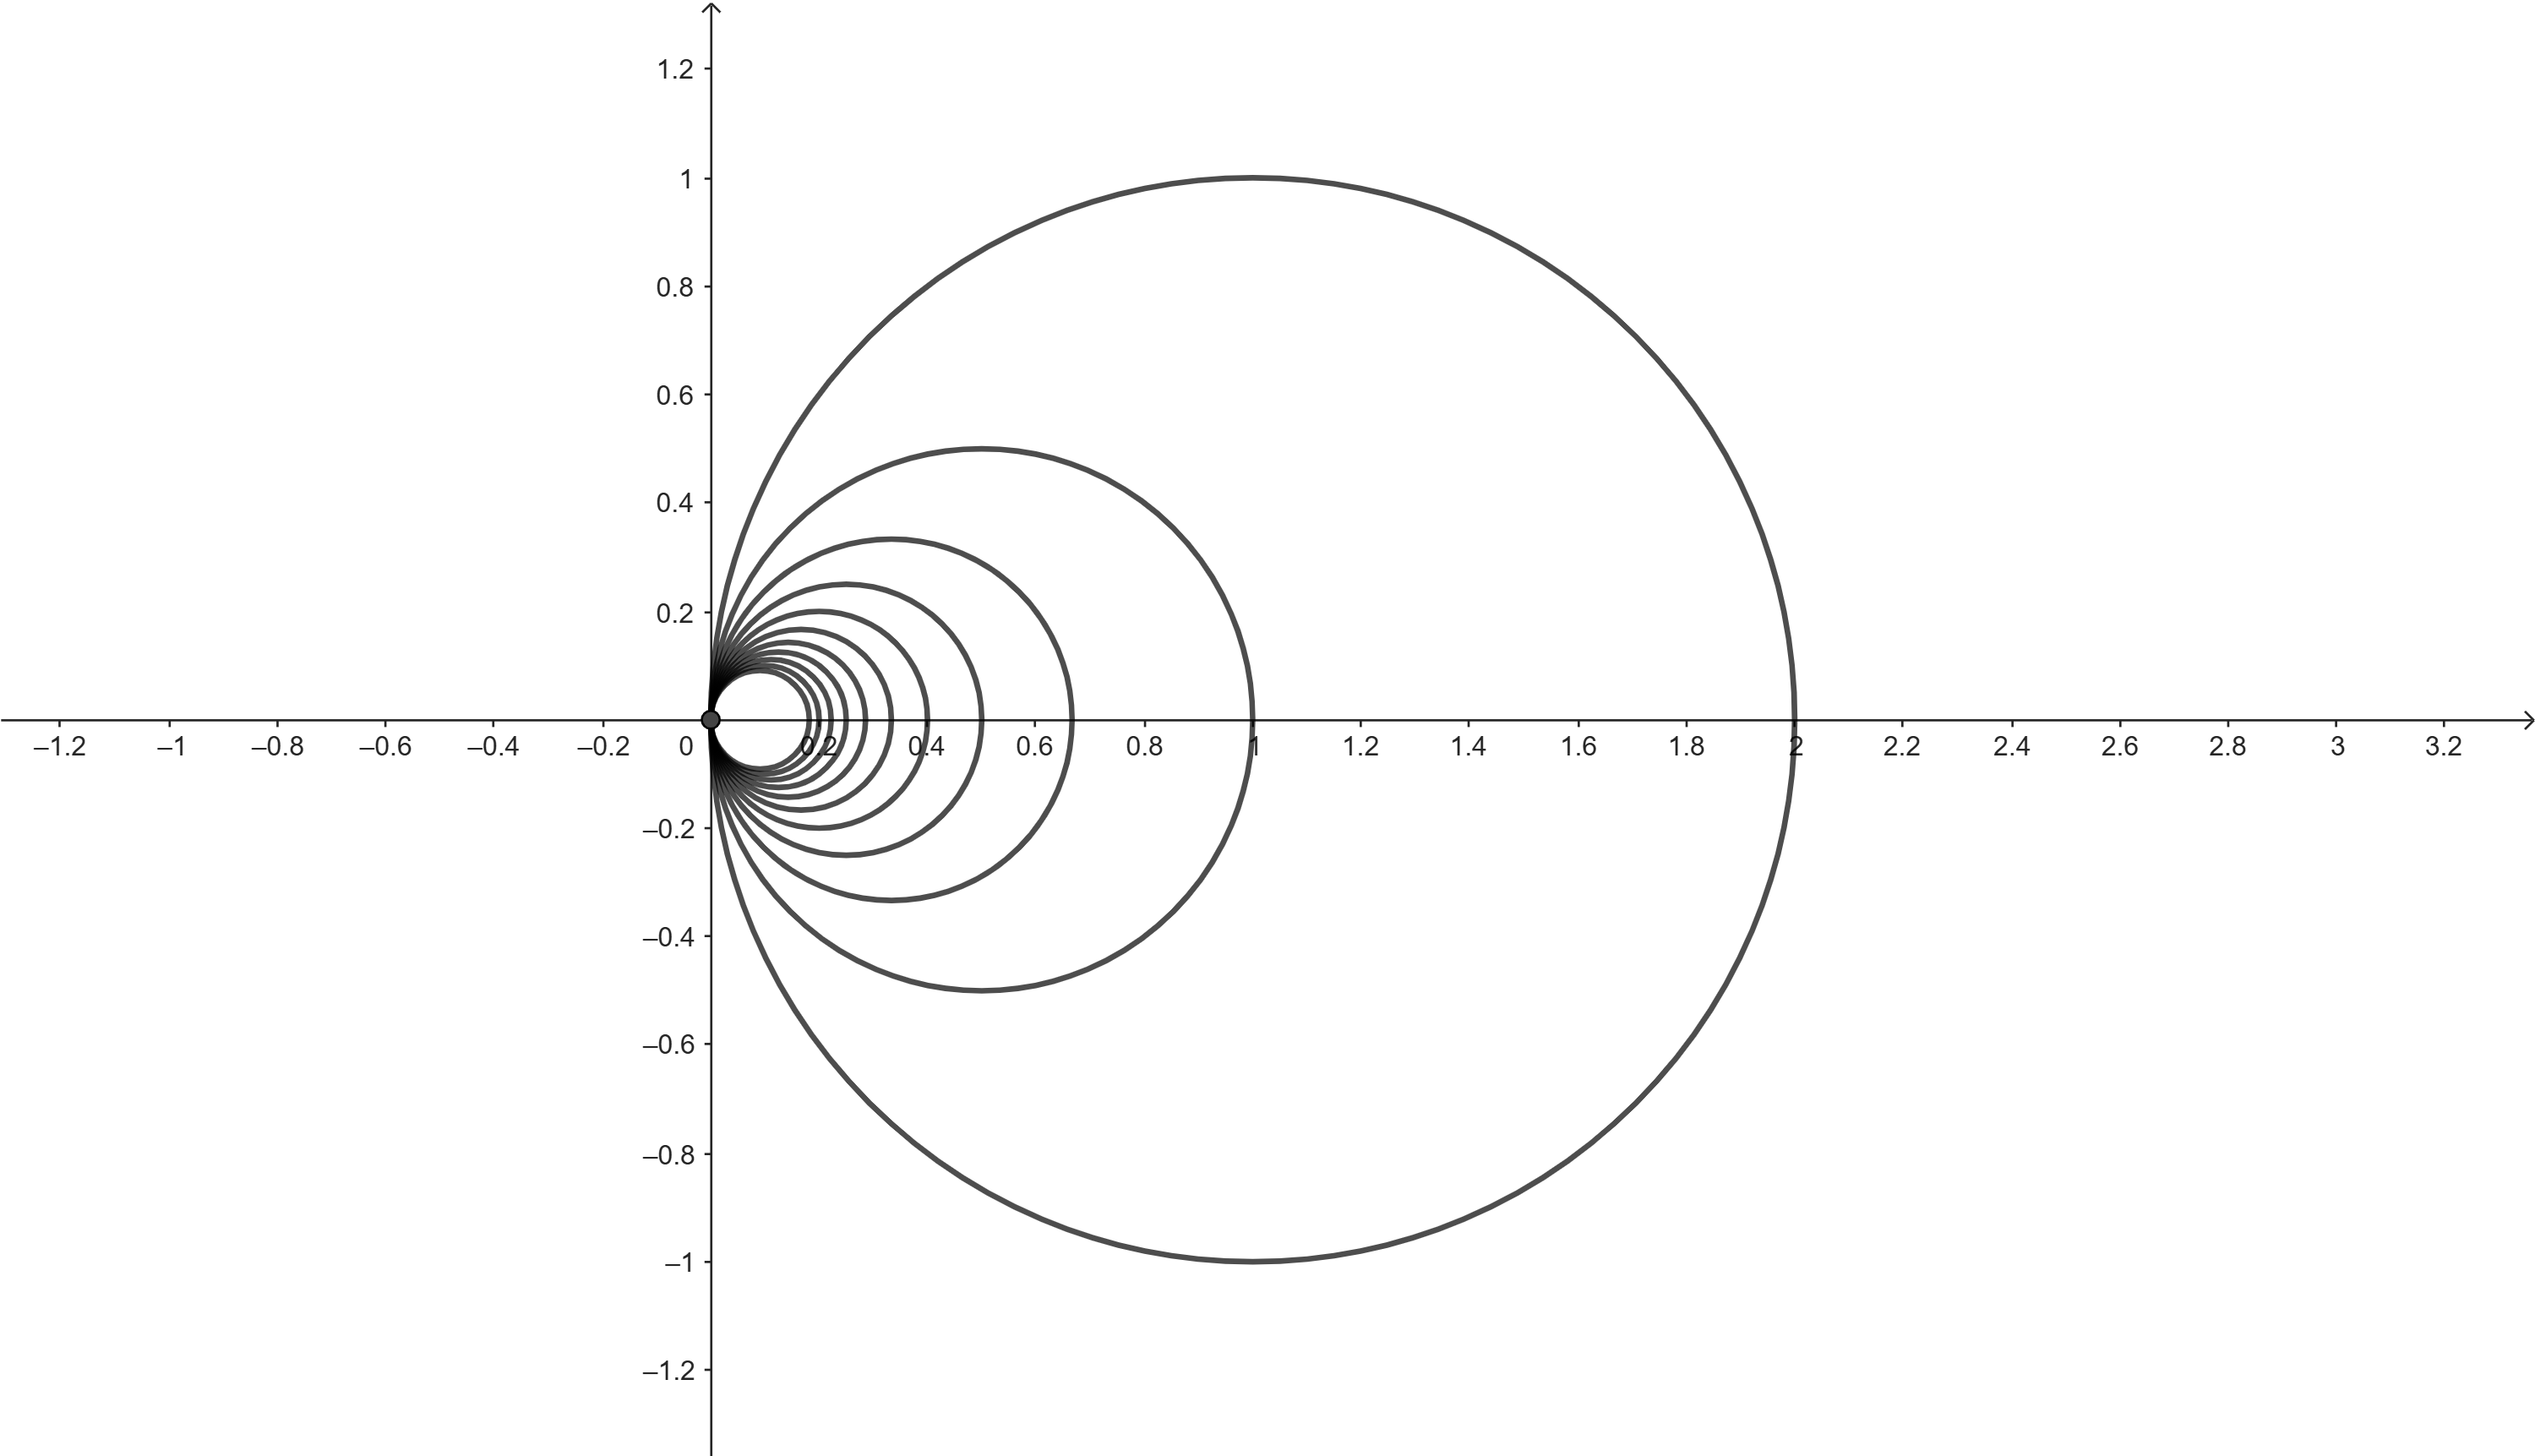
\includegraphics[width=0.8\textwidth]{conteudo/fig-brinco-havaiano.png}
	\caption{Brinco Havaiano}
	\label{fig: brinco havaiano}
\end{figure}





\begin{titlemize}{Lista de consequências}
	\item \hyperref[recobrimento-1-conexo-prop]{Teorema dos recobrimentos 1-conexos};\\ %'consequencia1' é o label onde o conceito Consequência 1 aparece
	%\item \hyperref[]{}
\end{titlemize}


%%% Local Variables:
%%% mode: LaTeX
%%% TeX-master: "../Alg.Top-Wiki"
%%% End:
